\section{Implementation}
\label{section:implementation}
The N-Queens hill climbing solution presented in this paper was implemented in AngularJS, in order to more easily
develop the solution, and quickly prototype a UI built for exploring the problem. The solution presented here is an
excellent source for learning Hill Climbing because of certain extensions made to the original assignment, and the
focus on interaction.

\subsection{Application Structure}
The application itself is stored as AngularJS code served by a Node.js API. The project is built with modern practices,
so \texttt{package.json} describes the Node.js dependencies and project configuration and \texttt{bower.json} describes
the client-side dependencies.

\subsubsection{Setup}
To run the project, the following must be installed on the machine:
\texttt{node}\cite{node}, \texttt{npm}\cite{npm}, \texttt{bower}\cite{bower}.

Then use \texttt{npm} and \texttt{bower} to install the dependencies:

\begin{lstlisting}
# Install server dependencies
npm install

# Install client JS dependencies
bower install
\end{lstlisting}

\subsubsection{Running}
The project is setup to run easily, using scripts defined in \texttt{package.json}. Simply run the following:

\begin{lstlisting}
npm start
\end{lstlisting}

Then browse to the page at \url{http://localhost:8080}

\subsubsection{Javascript Files}
The core of the project is in the Javascript files under \texttt{n-queens/public/js}. Here, each folder and file within
is described:

\begin{description}
  \item[/controllers]   Contains business logic wiring up Hill Climbing backend code to user interaction in the UI
  \begin{description}
    \item[BruteCtrl.js]             Manages the brute force page
    \item[ClimbCtrl.js]             Manages the Hill Climbing page
  \end{description}
  \item[/filters]       Contains AngularJS filters, which help transform data/text in the UI
  \begin{description}
    \item[TimeFilters.js]           Filters for showing timespans in the UI
  \end{description}
  \item[/services]      Contains models and core code implementing the Hill Climbing algorithms
  \begin{description}
    \item[HillClimbingService.js]   Implements the Hill Climbing algorithm
    \item[NQUeensService.js]        Abstractions around an N*N board with a Queen in each column
  \end{description}
  \item[app.js]         Declares the AngularJS application, including dependencies
  \item[appRoutes.js]   Defines the app routes, connecting URLs to a controller and view
\end{description}

\subsection{N-Queens Modelling}
One of the critical parts of the assignment is modelling the N-Queens board. This solution used a board-focused model,
with the board stored as a 2D array of objects representing each cell. The cell object stores a number of fields:

\begin{description}
\item[queen] Whether or not a queen is in the cell now
\item[initialQueen] Whether or not a queen started out in the cell in the initial board
\item[opportunity] Number of attacking queens if the queen in that row were moved to this cell
\item[row] Reverse lookup of where the cell is
\item[col] Reverse lookup of where the cell is
\end{description}

The board object itself resides inside a larger object containing metadata about the board state:

\begin{description}
\item[board] The board with N*N cells as described above
\item[queens] Denormalized store of the queens in the board
\item[best] The best H achieved while hill climbing with this board
\item[h] Current number of pairs of attacking queens in the board
\item[iterations] How many queen moves have been made against this board
\item[start] Timestamp when hill climbing (or random brute force)  began
\item[end] Timestamp when hill climbing (or random brute force) ended
\end{description}

In hindsight, the 2D N*N array representing the board was redundant with the much simpler 1D N array of queens.
Simplifying the model in this way could save prescious computation time, improving overall performance.

\subsection{Web Application}
The web UI has a tab for each of the implemnted use cases: Hill Climbing and Brute Force. This section describes the
major aspects of the UI.

\subsubsection{Board Generation}
In the upper right on both tabs, the user can generate a random board with 1 to 16 queens (N). On the Brute Force tab,
the user can choose how many random boards to generate in a brute search for a winning solution.

\subsubsection{Board Display}
The board is shown as a table with icons showing where the queens are \ref{fig:ui}. After evaluation on either tab, two sets of
queens will be shown. White queens show where the queens were initially, and black queens show where they ended up.
A legend at the bottom of the screen shows the number of pairs of attacking queens for the initial and final queen
positions.

\begin{figure}[ht!]
\centering
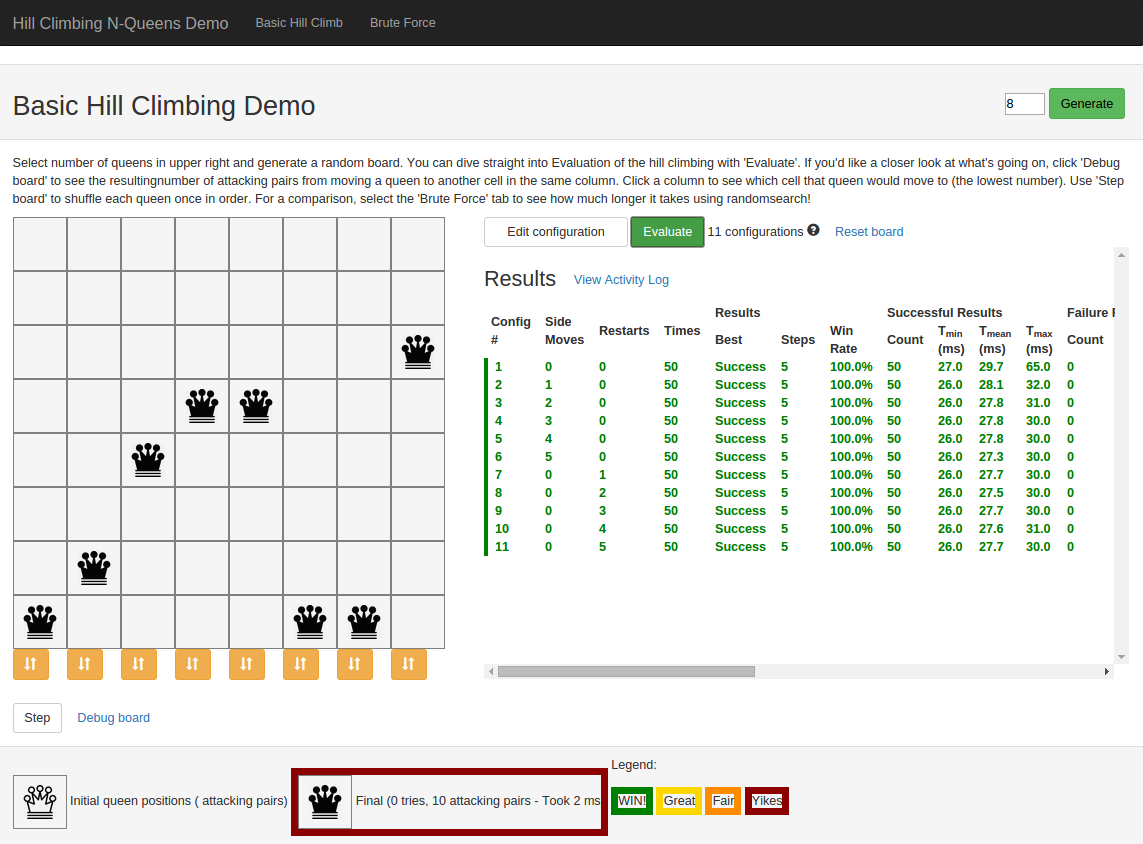
\includegraphics[width=90mm]{img/ui.png}
\caption{The assignment was solved with a focus on user interaction for the purposes of learning}
\label{fig:ui}
\end{figure}

\subsubsection{Learning Hill Climbing}
A neat feature of the UI is the ability to ``Debug board" to see what the prospective H would be after moving a queen to
another cell in the same column. To build on this, the user can choose to automatically move the best queen with ``Step,"
or move a queen in a particular column by clicking the orange button under that column.

\subsubsection{Evaluation}
On the Hill Climbing tab, the user can choose to ``Edit Configuration," specifying a list of board configurations to
evaluate \ref{fig:config}. Each configuration can specify a number of sideways moves allowed, random restarts allowed, and how many
times to try each configuration. Once they've set up a configuration, the user can choose to evaluate the displayed
board. The results will then be shown under ``View Results." The ``Activity Log" section can be used to help debug and
understand what the algorithm is doing.


\begin{figure}[ht!]
\centering
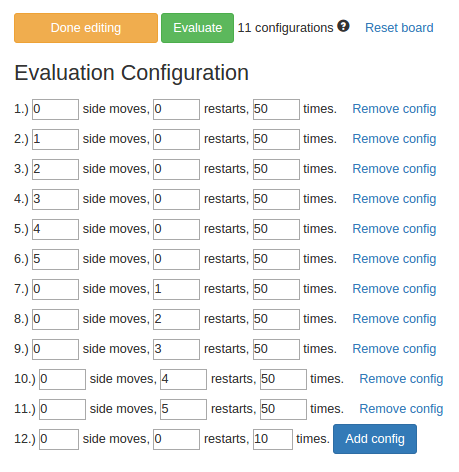
\includegraphics[width=90mm]{img/config.png}
\caption{The user can manage a list of configurations to evaluate. This is useful for comparing results with different parameters.}
\label{fig:config}
\end{figure}
